% This is a Basic Assignment Paper but with like Code and stuff allowed in it, there is also url, hyperlinks from contents included. 

\documentclass[11pt]{article}

% Preamble

\usepackage[margin=1in]{geometry}
\usepackage{amsfonts, amsmath, amssymb}
\usepackage{fancyhdr, float, graphicx}
\usepackage[utf8]{inputenc} % Required for inputting international characters
\usepackage[T1]{fontenc} % Output font encoding for international characters
\usepackage{fouriernc} % Use the New Century Schoolbook font
\usepackage[nottoc, notlot, notlof]{tocbibind}
\usepackage{listings}
\usepackage{xcolor}
\usepackage{blindtext}
\usepackage{hyperref}
\hypersetup{
    colorlinks=true,
    linkcolor=black,
    filecolor=magenta,      
    urlcolor=cyan,
    pdfpagemode=FullScreen,
    }

\definecolor{codegreen}{rgb}{0,0.6,0}
\definecolor{codegray}{rgb}{0.5,0.5,0.5}
\definecolor{codepurple}{rgb}{0.58,0,0.82}
\definecolor{backcolour}{rgb}{0.95,0.95,0.92}

\lstdefinestyle{mystyle}{
    backgroundcolor=\color{backcolour},   
    commentstyle=\color{codegreen},
    keywordstyle=\color{magenta},
    numberstyle=\tiny\color{codegray},
    stringstyle=\color{codepurple},
    basicstyle=\ttfamily\footnotesize,
    breakatwhitespace=false,         
    breaklines=true,                 
    captionpos=b,                    
    keepspaces=true,                 
    numbers=left,                    
    numbersep=5pt,                  
    showspaces=false,                
    showstringspaces=false,
    showtabs=false,                  
    tabsize=2
}

\lstset{style=mystyle}

% Header and Footer
\pagestyle{fancy}
\fancyhead{}
\fancyfoot{}
\fancyhead[L]{\textit{\Large{SET Assignment 5 - Sequence Diagrams}}}
%\fancyhead[R]{\textit{something}}
\fancyfoot[C]{\thepage}
\renewcommand{\footrulewidth}{1pt}



% Other Doc Editing
% \parindent 0ex
%\renewcommand{\baselinestretch}{1.5}

\begin{document}

\begin{titlepage}
	\centering

	%---------------------------NAMES-------------------------------

	\huge\textsc{
		MIT World Peace University
	}\\

	\vspace{0.75\baselineskip} % space after Uni Name

	\LARGE{
		Software Engineering and Testing\\
		Second Year B. Tech, Semester 4
	}

	\vfill % space after Sub Name

	%--------------------------TITLE-------------------------------

	\rule{\textwidth}{1.6pt}\vspace*{-\baselineskip}\vspace*{2pt}
	\rule{\textwidth}{0.6pt}
	\vspace{0.75\baselineskip} % Whitespace above the title



	\huge{\textsc{
			Sequence Diagrams
		}} \\



	\vspace{0.5\baselineskip} % Whitespace below the title
	\rule{\textwidth}{0.6pt}\vspace*{-\baselineskip}\vspace*{2.8pt}
	\rule{\textwidth}{1.6pt}

	\vspace{1\baselineskip} % Whitespace after the title block

	%--------------------------SUBTITLE --------------------------	

	\LARGE\textsc{
		\centering
		Assignment 5
	} % Subtitle or further description
	\vfill

	%--------------------------AUTHOR-------------------------------

	Prepared By
	\vspace{0.5\baselineskip} % Whitespace before the editors

	\Large{
		Krishnaraj Thadesar \\
		Cyber Security and Forensics\\
		Batch A1, PA 20
	}


	\vspace{0.5\baselineskip} % Whitespace below the editor list
	\today

\end{titlepage}


\tableofcontents
\thispagestyle{empty}
\clearpage

\setcounter{page}{1}

\section{Aim}
Object Oriented Analysis and design using UML diagrams: Sequence diagram to show
message exchanges, using Open Source Tool.

\section{Objectives}
To learn the relationships and notions of Sequence diagram.

\section{Problem Statement}

\textbf{Draw Sequence for The Following Problem:} \\

\textit{The Purpose of an Attandence Assistant App is to help reduce the time taken for recording the attendance of a classroom in a school or college. The app will be able to record the attendance of a class in a matter of a few Seconds with minimum Energy Expended. It will record data on cloud, and be accessible to all the Teachers.}\\

The tasks we have to do are:
\begin{enumerate}
	\item You will have to identify the main entities (objects) for this system.
	\item You will have to find out the relationships between these objects.
	\item You will have to find the necessary attributes and functions that need to be associated
	      with each object to implement the functionality mentioned above.
	\item You will make a final comprehensive diagram show and all objects and their relations
	      along with their attributes and functions.
\end{enumerate}

\section{Theory}


\subsection{Sequence Diagram}

\subsubsection{What is a Sequence Diagram}

\begin{quotation}
	A sequence diagram is a type of interaction diagram in the Unified Modeling Language (UML) that represents the interactions between objects or components within a system in a time-based manner.
\end{quotation}

\subsubsection{What is the use of a Sequence Diagram}
\begin{enumerate}
	\item Visualizing the interactions and communication among objects or components of a system in a time-ordered manner.
	\item Identifying potential design issues and ambiguities that may arise in the system during its execution.
	\item Documenting and communicating the behavior of the system to developers, stakeholders, and users.
	\item Testing and validating the design of a system, by ensuring that the sequence of events or actions occur in the correct order.
\end{enumerate}
\subsubsection{Elements of a Sequence Diagram}

The elements of a sequence diagram include:
\begin{enumerate}
	\item \textbf{Objects or actors:} These are the components or entities that are involved in the interactions and communications within the system.
	\item \textbf{Lifelines:} These are the vertical dashed lines that represent the lifespan of an object or component within the system.
	\item \textbf{Messages:} These are the arrows that represent the communications and interactions between objects or components within the system.
	\item \textbf{Activation bar:} This is a rectangle that is used to indicate the time interval during which an object or component is performing an action or task.
	\item \textbf{Constraints and loops:} These are used to specify conditions and repetitions in the interactions and communications within the system.
	\item \textbf{Combined fragment:} This is used to represent complex interactions or conditions in a sequence diagram.
\end{enumerate}

Here are the elements of a Sequence Diagram:
\begin{figure}[H]
	\centering
	\includegraphics[width=.7\textwidth]{sqdiagm1.png}
	\caption{Elements of a Sequence Diagram}
\end{figure}
\begin{figure}[H]
	\centering
	\includegraphics[height=.3\textwidth]{sqdiagm2.png}
	\caption{Elements of a Sequence Diagram}
\end{figure}
\begin{figure}[H]
	\centering
	\includegraphics[width=.45\textwidth]{sqdiagm4.png}
	\caption{Messages in a Sequence Diagram}
\end{figure}
\begin{figure}[H]
	\centering
	\includegraphics[width=.55\textwidth]{sqdiagm3.png}
	\caption{Messages in a Sequence Diagram}
\end{figure}

\subsubsection{Sequence Diagram for the Problem Statement}

\begin{figure}[H]
	\centering
	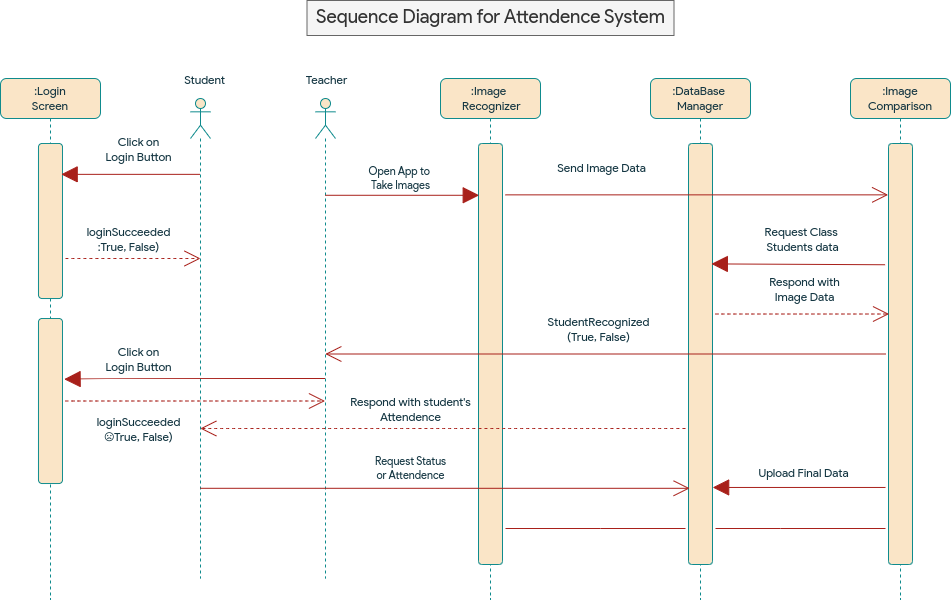
\includegraphics[height=1.2\textwidth]{Sequence Diagram.drawio.png}
	\caption{Sequence Diagram for the Problem Statement}
	\label{fig:state_diagram_problem_statement}
\end{figure}

\clearpage

\section{Platform}
\textbf{Operating System}: Arch Linux x86-64 \\
\textbf{IDEs or Text Editors Used}: Visual Studio Code\\
\textbf{External Programs for Diagrams} : Draw.io\\


\section{Conclusion}
Thus, we learnt about Sequence diagrams and their usage in detail.
\clearpage

\section{FAQ}

\begin{enumerate}
	\item \textbf{Give the significance of dynamic diagrams in UML.}\\

	      \begin{enumerate}
		      \item They help to visualize and understand the flow of interactions between objects and components within a system.
		      \item They help to identify potential bottlenecks and performance issues in the system.
		      \item They can be used to verify and validate the correctness of the system's behavior and interactions.
		      \item They can be used to communicate the behavior of the system to stakeholders, making it easier for them to understand and provide feedback.

	      \end{enumerate}
	\item \textbf{Explain any 2 terminologies used in Sequences diagrams.}\\

	      \begin{enumerate}
		      \item Lifeline: A lifeline represents an object or component that participates in the interaction. It is represented by a vertical line that extends down the diagram, with an optional name and activation bar. The activation bar represents the period of time during which the object or component is active.

		      \item Message: A message is a communication between two lifelines. It represents a request from one object or component to another. Messages are represented by horizontal arrows between lifelines, with an optional name and parameters.
	      \end{enumerate}
	\item \textbf{Explain the message passing in Sequence diagram.}\\

	      Message passing is a key concept in sequence diagrams. It is used to model the communication and interaction between different objects or components in a system. In a sequence diagram, message passing is represented using arrows between lifelines, with the arrows labeled with the message that is being passed.\\

	      When an object or component sends a message to another object or component, it can trigger a response from the receiving object or component. The response can be a return message, an exception, or a change in the state of the receiving object or component. The sequence diagram can include loops, conditionals, and other control structures to model the flow of messages and interactions.

	\item \textbf{Draw the Sequence diagram for the following scenario: Conduction of the National Event: HACK-MITWPU for Technical event at MITWPU
		      university.}\\


\end{enumerate}

\end{document}